\documentclass[../mathNotesPreamble]{subfiles}
\begin{document}
%\relscale{1.4}
  \section{6.2: Regions Between Curves}

  \begin{defn*}[Area of a Region Between Two Curves]
    Suppose $f$ and $g$ are continuous functions with $f(x)\geq g(x)$ on the interval $\sbrkt{a,b}$. The area of the region bounded by the graphs of $f$ and $g$ on $\sbrkt{a,b}$ is
      \[A=\int_a^b \parens{f(x)-g(x)}\,dx.\]
  \end{defn*}
  \begin{center}
    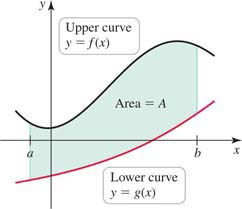
\includegraphics[width=0.3\linewidth]{../images/briggs_06_02/fig06_11}
  \end{center}

  \begin{ex*}
    Consider the region bounded by the curves $y=\cos(x)$ and $y=1-\cos(x)$, $0\leq x\leq \pi$.  Set up the integral(s) representing the area of this region.
  \end{ex*}
  \begin{flushright}
    \begin{tikzpicture}
      \begin{axis}[
        grid style={line width=0.3pt, draw=gray!60},
        axis lines=center,
        axis line style={black,->},
        xmin=-3.14/2, xmax=3.14*2,
        ymin=-1.5, ymax=2.5,
        xtick={0.0, 1.5707963267948966, 3.141592653589793, 4.71238898038469},
        xticklabels={0, $\pi/2$, $\pi$, $3\pi/2$},
        ytick={-2,-1,...,2},
        ticklabel style={font=\footnotesize,inner sep=0.5pt,fill=white,opacity=0.5, text opacity=1},
        every axis plot/.append style={line width=0.95pt, color=blue, samples=100},
        width=0.45\linewidth, height=0.3\linewidth
        ]
        \addplot[->, name path=A, ClemsonPurple] expression[domain=-pi/2:2*pi]{1-cos(deg(x))};
        \addplot[->, name path=B, ClemsonOrange] expression[domain=-pi/2:2*pi]{cos(deg(x))};
        \addplot[fill=HowardsRock!55, opacity=0.75] fill between[of=A and B, soft clip={domain=0:3.14}];
      \end{axis}
    \end{tikzpicture}
  \end{flushright}
  \pagebreak

  \begin{ex*}
    Find the area of the region by integrating with respect to $x$.
  \end{ex*}
    \begin{flushright}
    \begin{tikzpicture}
      \begin{axis}[
        grid style={line width=0.3pt, draw=gray!60},
        axis lines=center,
        axis line style={black,->},
        xmin=-0.25, xmax=1.5,
        ymin=-0.25, ymax=2.5,
        xtick={0,1},
        ticklabel style={font=\footnotesize,inner sep=0.5pt,fill=white,opacity=0.5, text opacity=1},
        every axis plot/.append style={line width=0.95pt, color=blue, samples=100},
        width=0.45\linewidth, height=0.3\linewidth
        ]
        \addplot[-, name path=A, black] expression[domain=0:1]{2-x} node[black, pos=0.5, above right] {$y=2-x$};
        \addplot[-, name path=B, red] expression[domain=0:1]{x} node[black, pos=0.5, below right] {$y=x$};
        \addplot[fill=BlueRidge!50, opacity=0.5] fill between[of=A and B, soft clip={domain=0:1}];
        \addplot[soldot, black] coordinates{(0,2)} node[above right, font=\normalsize] {$(0,2)$};
        \addplot[soldot, black] coordinates{(1,1)} node[above right, font=\normalsize] {$(1,1)$};
      \end{axis}
    \end{tikzpicture}
  \end{flushright}
  \vspace*{\stretch{1}}

  \begin{ex*}
    Find the volume of the solid whose base is bounded by the graphs of $y=x+1$ and 
$y=x^2-1$, with the cross sections in the shape of rectangles of height $2$ taken perpendicular to the $x$-axis.
  \end{ex*}
  \begin{flushright}
    \begin{tikzpicture}
      \begin{axis}[
        grid style={line width=0.3pt, draw=gray!60},
        axis lines=center,
        axis line style={black,->},
        xmin=-2.25, xmax=2.25,
        ymin=-1.5, ymax=3.5,
        ticklabel style={font=\footnotesize,inner sep=0.5pt,fill=white,opacity=0.5, text opacity=1},
        every axis plot/.append style={line width=0.95pt, color=blue, samples=100},
        width=0.45\linewidth, height=0.3\linewidth
        ]
        \addplot[-, name path=A, ClemsonPurple] expression[domain=-2.5:2.5]{x+1};
        \addplot[-, name path=B, ClemsonOrange] expression[domain=-2.5:2.5]{x^2-1};
        \addplot[fill=HowardsRock!55, opacity=0.75] fill between[of=A and B, soft clip={domain=-1:2}];
      \end{axis}
    \end{tikzpicture}
  \end{flushright}
  \vspace*{\stretch{1}}
  \pagebreak

  \begin{defn*}[Area of a Region Between Two Curves with Respect to $y$]
    Suppose $f$ and $g$ are continuous functions with $f(y)\geq g(y)$ on the interval $\sbrkt{c,d}$. The area of the region bounded by the graphs $x=f(y)$ and $x=g(y)$ on $\sbrkt{c,d}$ is
      \[A=\int_c^d \parens{f(y)-g(y)}\,dy.\]
  \end{defn*}

  \begin{ex*}
    Find the area of the region bounded by $x=3y$, and $x=y^2-10$
  \end{ex*}
  \begin{tasks}[after-item-skip=\stretch{1}, label=](1)
    \task 
      by integrating with respect to $x$
    \task 
      by integrating with respect to $y$
  \end{tasks}
  \vspace*{\stretch{1}}
  \pagebreak

  \begin{ex*}
    Find the area of the region bounded by $y=x^3$, and $y=\sqrt{x}$
  \end{ex*}
  \begin{tasks}[after-item-skip=\stretch{1}, label=](1)
    \task 
      by integrating with respect to $x$
    \task 
      by integrating with respect to $y$
  \end{tasks}
  \vspace*{\stretch{1}}
  \pagebreak

  \begin{ex*}
    Find the area of the region bounded by $y=4\sqrt{2x}$, $y=2x^2$, and $y=-4x+6$
  \end{ex*}
  \begin{flushright}
    \begin{tikzpicture}
      \begin{axis}[
        grid style={line width=0.3pt, draw=gray!60},
        axis lines=center,
        axis line style={black,->},
        xmin=-0.125, xmax=2.5,
        ymin=-0.75, ymax=9,
        xmajorticks=false, 
        ymajorticks=false,
        ticklabel style={font=\footnotesize,inner sep=0.5pt,fill=white,opacity=0.5, text opacity=1},
        every axis plot/.append style={line width=0.95pt, color=blue, samples=100},
        width=0.45\linewidth, height=0.4\linewidth
        ]
        \addplot[-, name path=A, ClemsonPurple] expression[domain=0:2.25]{4*sqrt(2*x)};
        \addplot[-, name path=B, ClemsonOrange] expression[domain=0:2.25]{2*x^2};
        \addplot[-, name path=C, black] expression[domain=-1:2.25]{-4*x+6};
        \addplot[fill=HowardsRock!55, opacity=0.75] fill between[of=A and B, soft clip={domain=1:2}];
        \addplot[fill=HowardsRock!55, opacity=0.75] fill between[of=A and C, soft clip={domain=0.5:1}];
      \end{axis}
    \end{tikzpicture}
  \end{flushright}
  \pagebreak

\end{document}
